\chapter{UCNA Experiment}
\label{ch:UCNA_Experiment}
%%%%%%%%%%%%%%%%%%%%%%%%%%%%%%%%%%%%%%%%%%%%%%%%%%%%%%%%%%%%%%%%%%%%%%%%%%%%%%%
%%%%%%%%%%%%%%%%%%%%%%%%%%%%%%%%%%%%%%%%%%%%%%%%%%%%%%%%%%%%%%%%%%%%%%%%%%%%%%%
%%%%%%%%%%%%%%%%%%%%%%%%%%%%%%%%%%%%%%%%%%%%%%%%%%%%%%%%%%%%%%%%%%%%%%%%%%%%%%%

The UCNA Experiment is a rather mature experiment, having taken data from
2007-2013, that aims to precisely determine a value of $A_{0}$, the neutron
$\beta$-decay asymmetry parameter. Here a description of the experimental
apparatus is given, as well as previous measurements
of $A_{0}$ from other experiments for comparison.


\section{Overview}
\label{sec:Overview}

The goal of UCNA is to produce UCN in a solid deuterium source which is fed
neutrons via a spallation source at the end of an $800$ MeV
proton beam. These UCN are then guided towards a material trap where they can
decay. During travel, the UCN pass through a series of polarizing magnets
which allows the experimenter to control the spin state of the neutrons in
the trap during any run. Utilizing a strong $~1$~T magnetic field in the
decay volume, decay electrons are guided towards detectors at either end of
the decay volume where their energy can be reconstructed. From knowledge about
the initial direction and the energy of the neutron, one can construct an
energy dependent asymmetry and determine a value for $A_{0}$.

%%%%%%%%%%%%%%%%%%%%%%%%%%%%%%%%%%%%%%%%%%%%%%%%%%%%%%%%%%%%%%%%%%%%%%%%%%%%%%%
%%%%%%%%%%%%%%%%%%%%%%%%%%%%%%%%%%%%%%%%%%%%%%%%%%%%%%%%%%%%%%%%%%%%%%%%%%%%%%%
\section{Ultracold Neutron Source and Guide System}
Detailed descriptions of the UCN source can be found in
\cite{saunders2004demonstration,morris2002measurements,saunders2013performance}, with
more recent improvements given in \cite{ito2017performance}.

The creation of UCN begins with delivery of protons from the 800~MeV proton
accelerator operated in pulsed mode, with pulses repeated at a rate of 0.2~Hz.
The protons strike a helium-cooled tungsten target (12~cm long) and produce
spallation neutrons at roughly 20~MeV. The spallation target is surrounded by
a room temperature beryllium reflector to help direct as many neutrons as
possible towards the UCN source. The solid deuterium ($\mathrm{SD}_2$) UCN source
is located directly above the tungsten target and is housed in a liquid helium
cooled cryostat. Prior to entering the $\mathrm{SD}_2$ source, neutrons
pass through a 1~cm thick moderator made of polyethylene beads cooled with the boil off gas
from the cooling of the $\mathrm{SD}_2$ source in the cryostat.

The $\mathrm{SD}_2$ source is a cylinder 19.7~cm in diameter and 5.7~cm tall. There
are a collection of ``fins'', or vertical teeth-like structures, located in
the bottom of the aluminum cryostat to increase the surface area of contact between the
$\mathrm{SD}_2$ and the liquid helium cooled surface. The surface of the cryostat
is coated with beryllium to reflect as many UCN as possible within the UCN source. Above
the $\mathrm{SD}_2$ is a flapper valve which opens to let UCN out of the source and
prevents UCN from re-entering the $\mathrm{SD}_2$ to reduce upscattering and loss of UCN.

Once a UCN passes the flapper, it is guided along a 1~m vertical guide coated with $^{58}\mathrm{Ni}$.
At this point, the UCN enter stainless steel horizontal guides to be transported from
the biological shielding that surrounds the source. The higher 342~neV potential of the
the $^{58}\mathrm{Ni}$ ensures that all neutrons which are capable of being guided by the
stainless steel (189 neV potential) are trapped at bottom of the vertical guide
\cite{saunders2013performance}. Upon looking at figure \ref{fig:guides}, one sees that
there are two $45\degree$ bends in the stainless steal guides to remove neutrons still
exceeding the UCN regime \cite{plaster2012}.

\begin{figure}[h]
  \centering
  \includegraphics[scale=0.48]{2-UCNAExperiment/experimentalSetup.png} 
  \caption{Schematic of guides and layout of the UCNA experiment.}
  \label{fig:guides}
\end{figure}

Once the UCN exit the shielding, they are guided along stainless steel guides
through a gate valve which allows for separation of the UCNA apparatus from the UCN
source while the proton beam is on, thus allowing for background measurements in
the spectrometer
during $\beta$-decay running conditions (proton beam operating, but void of UCN).
Beyond the gate valve is a 6~T pre-polarizing magnet (PPM). The purpose of the PPM
was to minimize the loss of UCN during transport through the Zr foil used to separate
the vacuum in the UCN source from the vacuum in the rest of the apparatus. The neutrons
are nominally polarized longitudinally after passing through the PPM's longitudinal field.

Beyond the PPM, the guides switch to electropolished copper (168 neV potential) to
maintain the initial polarization of the neutrons. Just downstream of the PPM
is the ``switcher'' valve. When the valve is open, the downstream guides are connected
to the guides coming from the PPM carrying UCN. Upon closing the switcher valve,
the downstream guides are redirected to a $^3\mathrm{He}$ 
UCN detector \cite{morris2009multi} used in polarimetry measurements.

Beyond the switcher,
the UCN are guided through the 7~T primary polarizing magnet (or AFP magnet). At this point
the guides switch to 100~cm of diamondlike carbon coated quartz guides \cite{mammei2010thin}
for passage through the Adiabatic Fast Passage (AFP) spin flipper \cite{holley2012high}. Again
the guides switch back to circular copper guides before coupling to a rectangular
(4~cm width $x$ 7~cm height) copper guide which transports the neutrons into the 1~T field
inside the Superconducting Spectrometer (SCS).


\section{Polarization}

\begin{figure}[h]
  \centering
  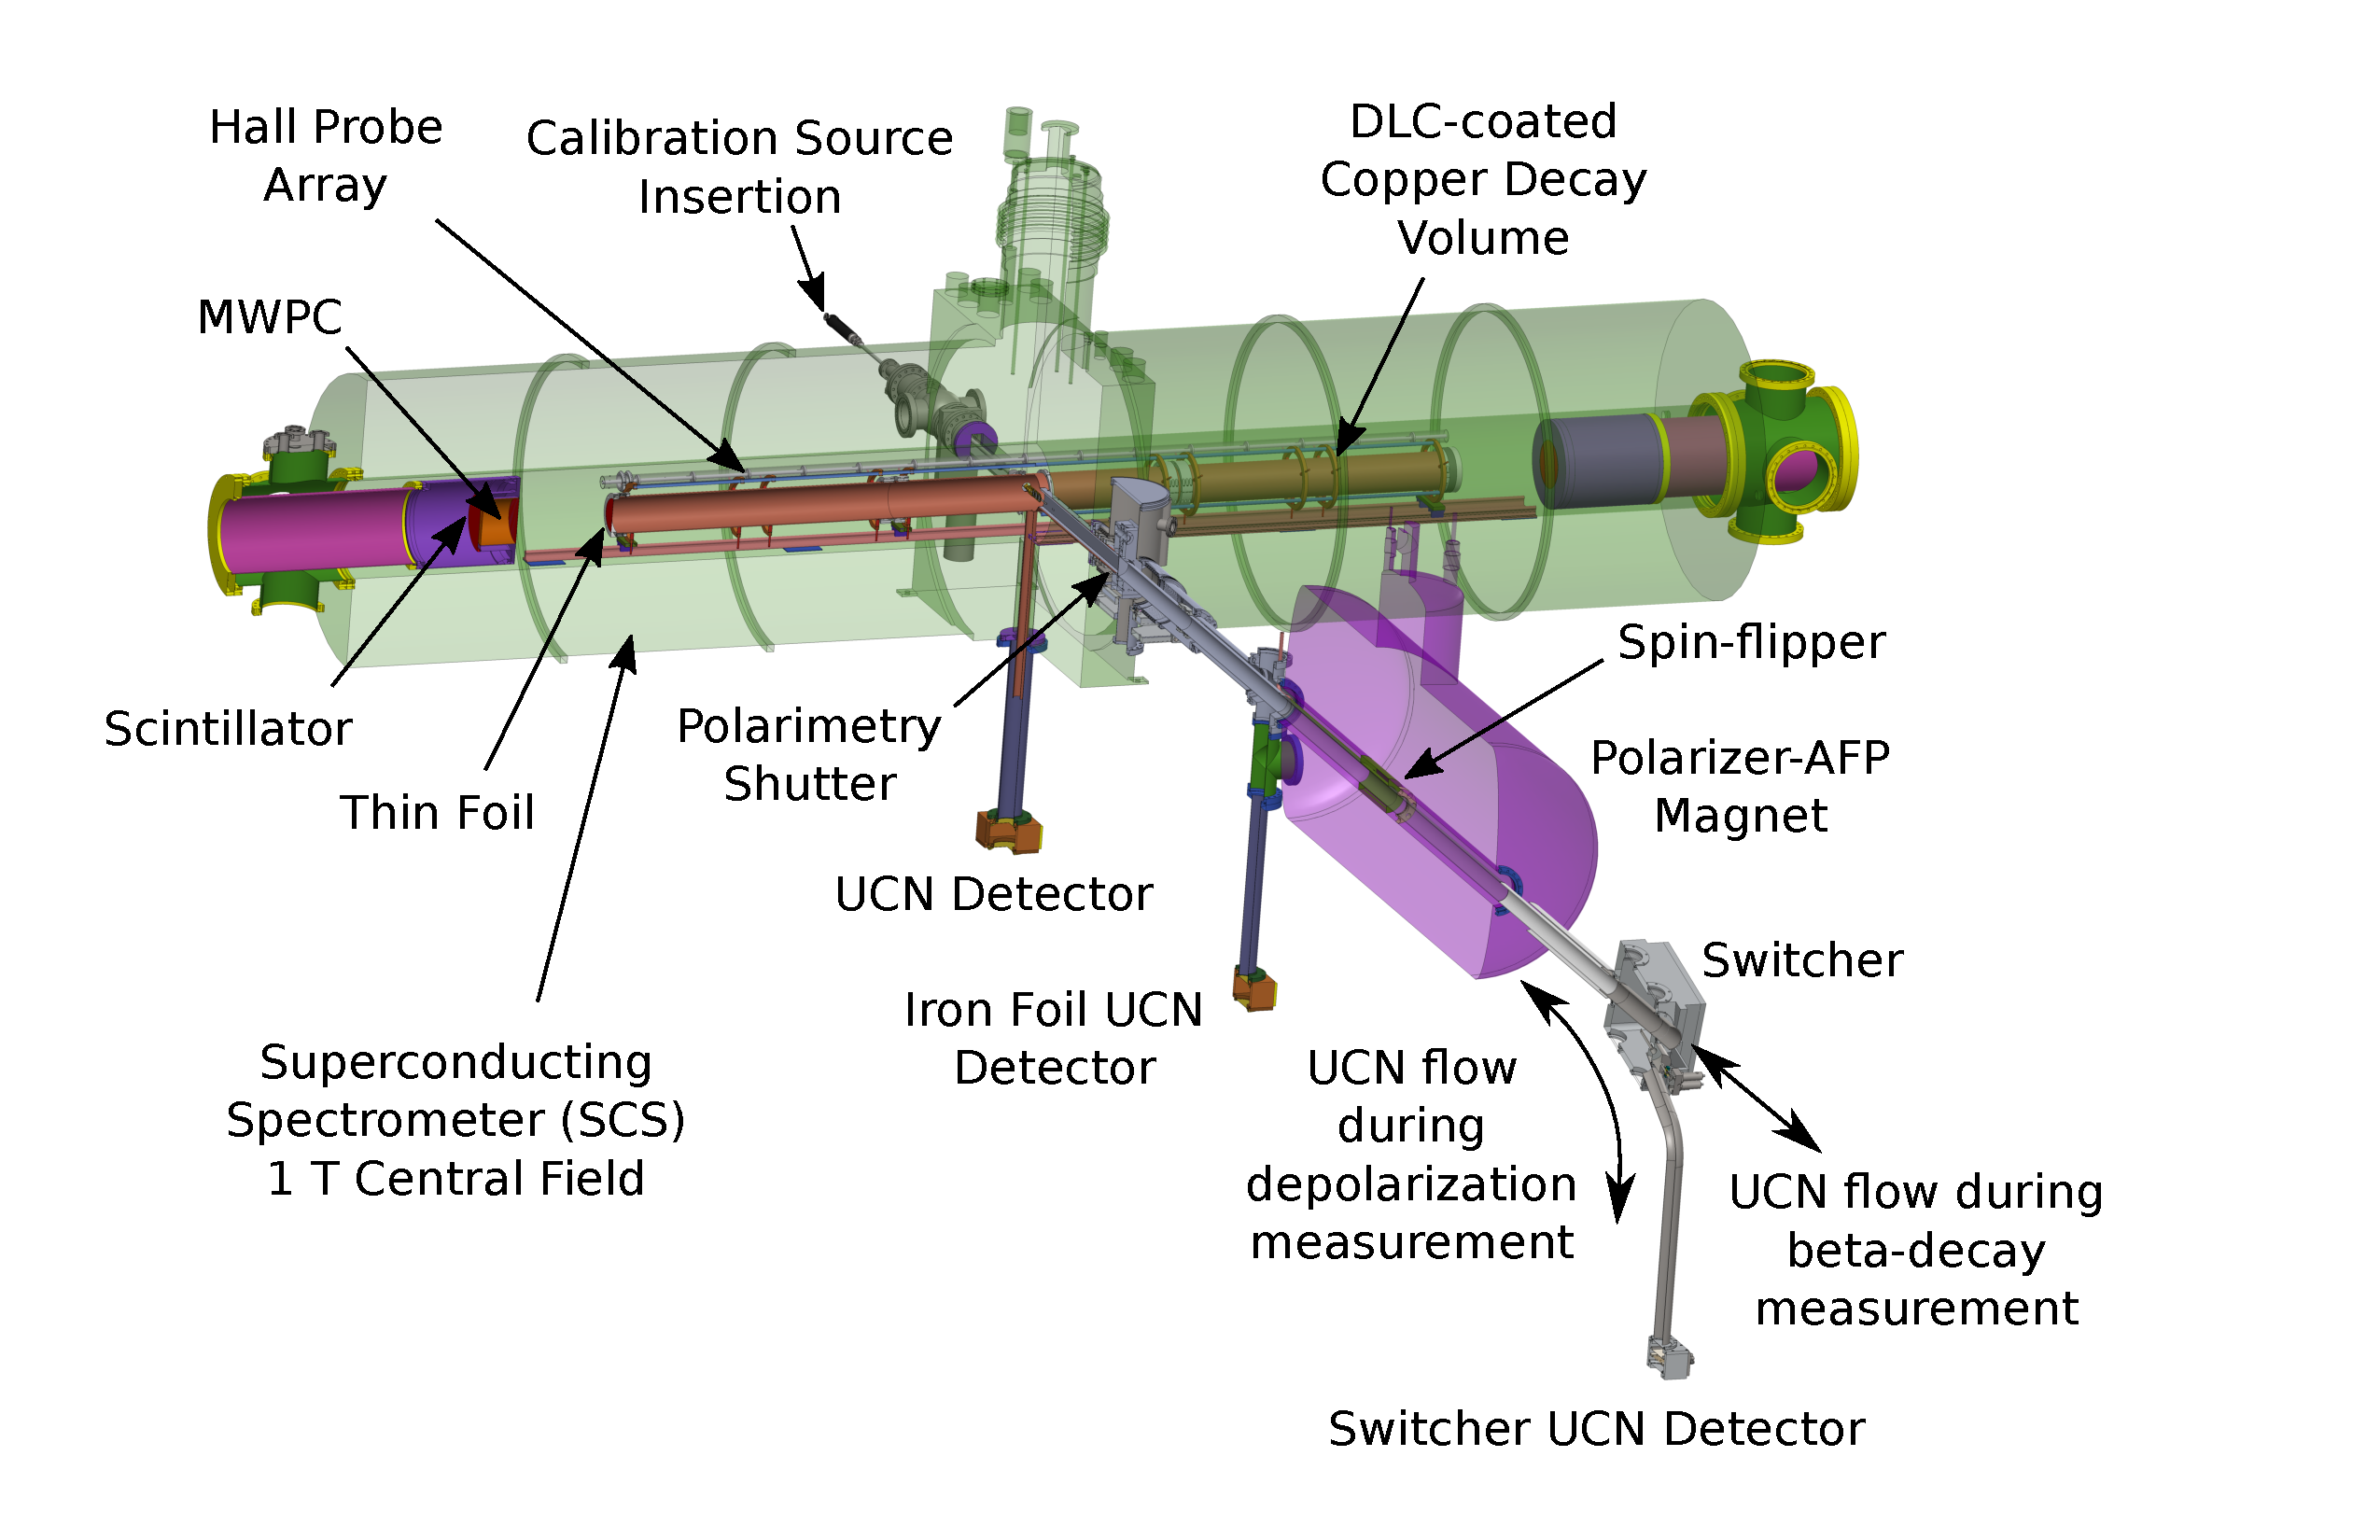
\includegraphics[scale=0.38]{2-UCNAExperiment/UCNAFig.pdf} 
  \caption{Schematic of guides and layout of the UCNA experiment.}
  \label{fig:setup}
\end{figure}

\section{Super-conducting Solenoidal Spectrometer}

\subsection{Decay Trap}

\subsection{Magnetic Field}


\section{Detector Packages}
\subsection{Multiwire Proportional Chamber}

\subsection{Scintillator}

\subsection{Calibration Scheme}

\subsection{PMT Gain Monitoring System}

\subsection{Muon Veto System}

\section{Data Acquisition}



%%%%%%%%%%%%%%%%%%%%%%%%%%%%%%%%%%%%%%%%%%%%%%%%%%%%%%%%%%%%%%%%%%%%%%%%%%%%%%







